\chapter{Theoretical Background}
\label{ch:theoretical-background}

\section{Ultrashort-pulse laser--matter interaction}
\label{sec:ch1-ultrashort}

Laser processing regimes are distinguished primarily by the pulse duration relative to the intrinsic relaxation times of the irradiated metal. In continuous-wave irradiation the delivered power is effectively steady in time, whereas in pulsed irradiation the energy arrives in discrete temporal packets. The ultrashort-pulse regime is reached when the pulse duration falls from the picosecond range into the femtosecond range, so that the laser excites the conduction electrons before the lattice can equilibrate with them \cite{Alexopoulou_2023,Zhang_2015}. Under these conditions the thermal response is no longer described adequately by a single Fourier temperature field, because the electron subsystem and the lattice subsystem evolve on distinct time scales during the early stages of irradiation \cite{Alexopoulou_2023,Zhang_2015}.

\begin{figure}[htbp]
  \centering
  \PublicFigureOmitted[0.85\linewidth]
  \caption{Long-pulse and ULP interaction with target material.\cite{Hamad_2016}}
  \label{fig:ch1-long-short-pulse}
\end{figure}

The two-temperature description follows from this temporal separation. The laser field is first absorbed by conduction-band electrons, which thermalise rapidly and then transfer energy to the lattice through electron--phonon coupling.
The resulting nonequilibrium state is the physical basis of the two-temperature model family documented in the literature \cite{Forsman_1998, ByskovNielsen_2011, Zhao_2014, Zhang_2015,Petrov_2021, Bulgakova_2021, Alexopoulou_2023, Takabe_2024, Shim_2026}.
In the present thesis, the governing formulation is referred to as the dual-parabolic two-temperature model (pTTM)\footnote{The thesis implements the pTTM variant throughout; see \S\ref{sec:ch1-ttm-variants} for a discussion of model selection.}. The nomenclature emphasises that both subsystems are described with Fourier-type conduction, while the electron and lattice temperatures remain distinct.

The parabolic two-step model (PTS) provides the starting point for this construction \cite{Alexopoulou_2023}. In the notation adopted throughout the chapter, it may be written as
\begin{subequations}\label{eq:ch1-pts}
  \begin{align}
    C_e(T_e)\frac{\partial T_e}{\partial t} & = - \nabla \cdot \mathbf{q}_e - G(T_e - T_l) + S \, , \label{eq:ch1-pts-e} \\
    C_l\frac{\partial T_l}{\partial t}      & = G(T_e - T_l) \, , \label{eq:ch1-pts-l}                                   \\
    \mathbf{q}_e                            & = - k_e \nabla T_e \, . \label{eq:ch1-pts-q}
  \end{align}
\end{subequations}
The studied model extends \eqref{eq:ch1-pts} by retaining Fourier heat conduction on the lattice subsystem as well, following the model implemented in Tsibidis et al. \cite{Fraggelakis_2021}.
In the axisymmetric setting used later in the monograph, the pTTM therefore takes the form
\begin{subequations}\label{eq:ch1-pttm}
  \begin{align}
    C_e \frac{\partial T_e}{\partial t}                                         & = \frac{1}{\varrho}\frac{\partial}{\partial \varrho}\left(\varrho \left[k_e \frac{\partial T_e}{\partial \varrho}\right]\right) + \frac{\partial}{\partial z}\left(k_e \frac{\partial T_e}{\partial z}\right) - G(T_e - T_l) + S(\varrho,z,t) \, , \label{eq:ch1-pttm-e} \\
    \left(C_l + H_m \, \delta[T_l - T_m]\right) \frac{\partial T_l}{\partial t} & = \frac{1}{\varrho}\frac{\partial}{\partial \varrho}\left(\varrho \left[k_l \frac{\partial T_l}{\partial \varrho}\right]\right) + \frac{\partial}{\partial z}\left(k_l \frac{\partial T_l}{\partial z}\right) + G(T_e - T_l) \, . \label{eq:ch1-pttm-l}
  \end{align}
\end{subequations}
Here \(C_e\) and \(C_l\) denote the electron and lattice heat capacities, \(k_e\) and \(k_l\) are the corresponding thermal conductivities, \(G\) is the electron--phonon coupling factor, \(H_m\) is the latent heat of melting, and \(S\) is the volumetric laser source term. The cylindrical coordinate \(\varrho\) is reserved for the radial coordinate, while \(z\) denotes the depth coordinate.
Equation \eqref{eq:ch1-pttm} is the canonical pTTM used in this thesis with the simplification \(H_m \rightarrow 0\) in the sub-ablation regime.

\begin{figure}[htbp]
  \centering
  \PublicFigureOmitted[0.85\linewidth]
  \caption{Schematic diagram of Ultra-short pulse laser interaction with metal. \(T_e\) and \(T_l\) are the electron and lattice temperatures, and \(T_0\) denotes the room temperature. \cite{Vaghasiya_2023}}
  \label{fig:ch1-ulp-metals}
\end{figure}

The subsequent simulations adopt the physical assumptions stated below. The geometry is taken to be axisymmetric, the azimuthal dependence is neglected, and the baseline simulations remain in the sub-ablation regime so that macroscopic material removal, moving boundaries, and vapour recoil are not part of the base pTTM.
Sublimation\footnote{Phase transition of the solid to the gaseous phase.} occurs when the lattice temperature for the
evaporation reaches sufficient energy to overcome the latent heat of fusion. The following temperature-dependent function should apply for a smoother
transition between the solid and liquid phases\cite{Grigoropoulos_1986}: (eq. 5 in Tsibidis et al. \cite{Tsibidis_2012})
\begin{equation}
  \delta [T_l - T_m] = \frac{1}{\sqrt{2\pi \Delta^2}} \exp \left\{ - \frac{(T_l - T_m)^2}{2 \Delta^2} \right\} \equiv G(T_l - T_m ; \mu = 0, \sigma^2 = \Delta^2) \ ,
\end{equation}
where the standard deviation, $\Delta$, is of the range $[10, 100]$ K, depending on the temperature gradient.
$T_m$ is the material's melting temperature. We focus on the solid-to-liquid transition (melting).
In solidification process, there is a sign change (i.e., $\delta[T] \coloneqq - G(T; \mu=0, \sigma^2=\Delta^2)$).
During the ultrafast heating of the material, the temperature of electrons and lattice rises so that temperature-dependent materials properties have a pivotal role
during the simulation \cite{Vaghasiya_2023}.

At the beginning of the (sub-)ablation process, the laser focus is on the initial surface of the material
($z_s = 0$), and the centre of the spot at $\varrho = 0$.
Material is removed as the ablation process progresses,
forming a new material surface, and the laser focus moves downward over time. Therefore, the
laser beam propagation equation can be expressed as follows (see Fig.~\ref{fig:ch1-rayleigh-sub} for concreteness):
\begin{equation}
  w(z,t) \coloneqq w_0 \sqrt{1 + \left(\frac{z - v t}{z_R}\right)^2},
  \label{eq:ch1-beam_propagation}
\end{equation}
where $w_0$ is the focus radius, $z_R$ is the Rayleigh length\footnote{The Rayleigh length is the distance along a laser beam's axis from the beam waist to the point where its cross-sectional area doubles due to diffraction.}, and $v$ is the downward focus speed.
The energy distributed inside the material is affected by the optical
penetration depth $\delta_s$ of the material and the electronic ballistic length $\delta_b$.\\

\noindent
Furthermore, the Rayleigh length can be calculated by the relation
\begin{equation}
  z_R = \frac{\pi  \cdot w_0^2}{\lambda \cdot M^2} \ ,
\end{equation}
where $w_0$ is the focused beam spot radius, $\lambda$ is the wavelength of the laser beam in vacuum, and $M^2$ is the laser beam quality factor.

\begin{figure}[htbp]
  \centering
  % Subfigure (a)
  \subfloat[Schematic representation of the Rayleigh length ($z_R$) and Rayleigh's criterion as applied to Gaussian beams. \cite{Penchev_2016}]{
    \PublicFigureOmitted[0.42\linewidth]
    \label{fig:ch1-rayleigh-sub}
  }
  \hfill
  % Subfigure (b)
  \subfloat[Conceptual diagram of the laser--material interaction mechanism. \cite{Dong_2019}]{
    \PublicFigureOmitted[0.42\linewidth]
    \label{fig:ch1-interaction-sub}
  }
  \caption{Overview of laser beam propagation characteristics and interaction regimes.}
  \label{fig:ch1-rayleigh_length_axisymmetric_laser}
\end{figure}

In the sub-ablation regime we investigate, the latent-heat term is
suppressed (i.e., $H_m \delta [T_l - T_m] \rightarrow 0$) and the model is interpreted as a conduction-dominated description of electron
heating and subsequent lattice equilibration.

\begin{figure}[H]
  \centering
  \PublicFigureOmitted[0.85\linewidth]
  \caption{The physical interaction process between ultrashort pulse laser and metal, including vaporisation, phase explosion, and supercritical-fluid trajectories. \cite{Song_2023}}
  \label{fig:ch1-laser-induced-trajectories}
\end{figure}

Figure~\ref{fig:ch1-laser-induced-trajectories} places this conduction-dominated model in the wider sequence of ultrashort laser--matter interaction. Absorption is followed by rapid electron heating, delayed lattice heating, and, at sufficiently high fluence, the onset of thermal damage. In the present chapter the retained ingredients are the optical response, the volumetric heat source, the thermophysical closures, and the model-selection rationale for the pTTM used in the threshold calculations.

\section{Optical properties, ballistic \& finite--thickness corrections}
\label{sec:ch1-absorption}

The laser source term in \eqref{eq:ch1-pttm} depends on the optical response of the irradiated metal.
Rethfeld et al. demonstrated that the ultrashort laser--metal interactions can be well described by laser--plasma ones \cite{Rethfeld_2002}. According to the Drude model for free electrons, $\epsilon$, the electrical permittivity (dielectric function) of metals modeled as a plasma, is expressed as
\begin{align*}
  \epsilon_{\text{(D)}}(t,\varrho,z) & =
  \epsilon_{\infty} - \frac{\omega_p^2}{\omega (\omega + i\gamma_D)} = \epsilon_1(t,\varrho,z)  + i \epsilon_2(t,\varrho,z)                                                                                                                                 \\
                                     & = \biggl( 1 - \frac{\omega_p^2(n_e) \tau_e^2(t,\varrho,z)}{1 + \omega^2 \tau_e^2(t,\varrho,z)} \biggr) + i \biggl(\frac{\omega_p^2(n_e) \tau_e(t,\varrho,z)}{\omega(1 + \omega^2 \tau_e^2(t,\varrho,z))} \biggr) \ ,
\end{align*}
where $\epsilon_\infty$ is the dc (zero frequency) dielectric function (in simple Drude model: $\epsilon_\infty = 1$), $\gamma_D\equiv 1/\tau_e$ the damping coefficient and
$\omega_p \equiv \sqrt{n_e e^2/ m_e \epsilon_0}$ the plasma frequency. The relationship between the refractive index, $n \in \mathbb{C}$, and the electrical permittivity, $\epsilon \in \mathbb{C}$, is given by\footnote{
  For corrections on the refractive index accounting for the nonlinear Kerr effect and its contributions on ultrafast dynamics, consult the study of Petrakakis et al. \cite{Petrakakis_2019}.
}
\begin{equation}
  \frac{c}{v} \equiv n = n_1 + i n_2 = \sqrt{\epsilon} = \sqrt{\epsilon_1 + \epsilon_2} \ ,
\end{equation}
where $c$ is the speed of light in vacuum; $v$ is the speed of light propagating through the material; $n_1$ is the normal refractive index;
and $n_2$ is the extinction coefficient.

\noindent
Thus, the $n_1$ and $n_2$ functions can be expressed as ($\| \epsilon \| \equiv \sqrt{\epsilon_1^2 + \epsilon_2^2}$)
\begin{subequations} \label{eq:ch1-coeffs_refractive_index}
  \begin{align}
    n_1(t,\varrho,z) & = \sqrt{\frac{1}{2} ( \epsilon_1 (t, \varrho, z) + \| \epsilon \| )}  \\
    n_2(t,\varrho,z) & = \sqrt{\frac{1}{2} ( -\epsilon_1 (t, \varrho, z) + \| \epsilon \| )}
  \end{align}
\end{subequations}
% [NOTE: report3 writes the refractive-index components as f_1 and f_2; Chapter 1 relabels them as n_1 and n_2 under the binding notation decision.]

The reflectivity and the absorption coefficient of the metal are determined by the following Fresnel expression
(FCA: free-carrier absorption)\footnote{
  The expressions in \ref{eq:ch1-fresnel} follow equations 6 in the work by Tsibidis et al. \cite{Tsibidis_2019} after reassigning $\omega \mapsto \omega_L$, $(n_1,n_2) \mapsto (n,k)$ and $z=z_s \mapsto z=0$.
}
\begin{subequations}\label{eq:ch1-fresnel}
  \begin{align}
    R(t,\varrho, z=z_s)                  & = \frac{(n_1(t, \varrho, z_s) - 1)^2 + n_2^2(t, \varrho, z_s)}{(n_1(t, \varrho, z_s) + 1)^2 + n_2^2(t, \varrho, z_s)}
    \label{eq:reflectivity_FCA}                                                                                                                                  \\
    \alpha_{(\text{FCA})}(t, \varrho, z) & = \frac{2 \omega}{c} n_2(t, \varrho, z), \qquad \delta_{opt} = \alpha^{-1}
    \label{eq:absorption_FCA}
  \end{align}
\end{subequations}
% [NOTE: report1 writes the free-carrier absorption coefficient as \(2\omega n_2/c\), whereas report3 rewrites the same quantity as \(4\pi n_2/\lambda\); the chapter keeps both equivalent forms explicit.]

However, the Drude model for metals, does not consider the inter-band transition and the Fermi distribution (e.g., d-band transitions in Au \cite{Schoenlein_1987}).

Vial et al. \cite{Vial_2005} pointed out that the Lorentz--Drude model \cite{Powell_1969} with five Lorentzian terms \cite{Rakic_1998} cannot match well experimental data around 2 eV for gold
(the energy for inter-band transition from d-band to Fermi level in gold is $\mathcal{E}_F - \mathcal{E}_d = 2.38$ eV).

They proposed an extended Drude model as follows:
\begin{equation}
  \epsilon_{\text{DL}} = \epsilon_\infty - \frac{\omega_p^2}{\omega (\omega + i \gamma_D)} - \frac{f\Omega_L^2}{(\omega^2 - \Omega_L^2) + i \Gamma_L \omega} \ ,
\end{equation}
where $\Omega_L$ and $\Gamma_L$ stand for the oscillator strength and the spectral width of the Lorentz oscillators, respectively, and $f$
is a weighting factor. With the values optimized for gold;
$\epsilon_\infty = 5.9673$, $\omega_p = 13.28$ THz, $\Omega_L = 4.085$ THz, $\Gamma_L= 0.659$ THz, and $f = 1.09$, their model fitted experimental data quite well in the range of 1.24--2.48 eV \cite{Vial_2005}.

Subfigures \ref{fig:ch1-R_vs_wavelength} and \ref{fig:ch1-alpha_vs_wavelength} compare $R$ and $\alpha$ for gold at room temperature (RT), respectively, among four optical models.
The extended Drude model performs best above $500$ nm, while the Lorentz-Drude model fits best at $\sim 250-500$ nm.

\begin{figure*}
  \centering
  \subfloat[Reflectivity at RT calculated by\\different optical models.]{
    \label{fig:ch1-R_vs_wavelength}
    \PublicFigureOmitted[0.30\textwidth]
  }
  \subfloat[Absorption coefficient at RT\\under different optical models.]{
    \label{fig:ch1-alpha_vs_wavelength}
    \PublicFigureOmitted[0.30\textwidth]
  }
  \subfloat[Time‑resolved evolution of reflectivity and absorption coefficient during pulsed laser irradiation.]{
    \label{fig:ch1-R_alpha_vs_t}
    \PublicFigureOmitted[0.30\textwidth]
  }
  \caption{Comparison of different optical models, adopted from Y. Ren et al. \cite{Ren_2011}.} % Add a main caption
  \label{fig:reflectivity-plots} % Label must come AFTER or INSIDE caption
\end{figure*}

In our work, the optical model is similarly extended by considering higher order Lorentz oscillations (5--6th order),
\begin{align}
  \epsilon(\omega)              & = \epsilon_{\mathrm{D}}(\omega) + \epsilon_{\mathrm{L}}(\omega) \, , \nonumber        \\
  \epsilon_{\mathrm{D}}(\omega) & = \epsilon_\infty -  \frac{f_0 \omega_p^2}{\omega^2 - i \Gamma_0(T_e, T_l) \omega}    \\
  \epsilon_{\mathrm{L}}(\omega) & = \sum_{k=1}^{K} \frac{f_k \omega_p^2}{\omega_k^2 + \omega^2 + i\Gamma_k \omega} \, ,
  \label{eq:ch1-lorentz-drude}
\end{align}
providing greater robustness across the spectral range of interest.
The Drude damping rate is defined as
\begin{equation}
  \Gamma_0(T_e, T_l)
  \coloneqq
  \Gamma_{\mathrm{base}}
  +
  B_L\!\left(
  \frac{A_e}{B_L} T_e^2 + T_l
  \right),
  \label{eq:ch1-drude-damping}
\end{equation}
where the quadratic term \(A_e T_e^2\) accounts for electron--electron
scattering, the linear term \(B_L T_l\) represents electron--phonon
scattering \cite[\S~II.C]{Lin_2008}.
For gold, the values adopted in the present study are
\(\Gamma_\mathrm{base} = \num{0.053}\,\si{\eV}\),
\((A_e/B_L)_{\mathrm{Au}} = \num{9.44e-5}\,\si{\per\kelvin}\) and
\(B_L|_{\mathrm{Au}} = \num{1.25e11}\,\si{\per\second\per\kelvin}\).

% [NOTE: report1 writes the interband correction as a single Lorentz term following Vial et al., whereas report3 gives the more explicit multi-oscillator Lorentz--Drude form.]

\begin{figure}[htbp]
  \centering
  \PublicFigureOmitted[0.60\linewidth]
  \caption{Three distinguished relaxation phases of optically excited electrons in metals.
    (a) Photon absorption within the optical penetration depth generates at $t=0$ nonequilibrium electrons which move with ballistic velocities into deeper parts of the sample.
    (b) At $t = \tau_\text{ph}$ electrons have equilibrated by electron-electron collisions forming a Fermi distribution with a well defined electron temperature $T_e$, and diffusive energy transport starts within the electron gas.
    (c) Through electron-phonon coupling the electrons come into equilibrium with the lattice at $t = \tau_\text{e-ph}$, energy transport now proceeds by lattice thermal diffusion. \cite{Hohlfeld_2000}}
  \label{fig:ch1-ballistic-electrons}
\end{figure}

The optical response also controls the characteristic penetration depth of deposited energy. In ultrashort irradiation this depth is not determined solely by \(\delta_{opt}\), because hot electrons can travel ballistically before complete thermalisation \cite{Hohlfeld_2000, Zhang_2015}.
The three-stage sequence shown in Figure~\ref{fig:ch1-ballistic-electrons} motivates the effective (ballistic) attenuation
\begin{equation}
  \alpha' = \frac{1}{\delta_{opt} + \delta_b} = \frac{\alpha}{1 + \alpha \delta_b} \, ,
  \label{eq:ch1-alpha-prime}
\end{equation}
where \(\delta_b\) denotes the ballistic length. The correction reduces the local deposition rate while preserving the correct local limit \(\alpha' \to \alpha\) when \(\delta_b \to 0\).
The finite film thickness \(L_z\) is incorporated through the multiplicative factor
\begin{equation}
  b(L_z;\alpha') = \frac{1}{1 - e^{-\alpha' L_z}} \, .
  \label{eq:ch1-thickness-factor}
\end{equation}
following the finite-thickness correction introduced by Chen et al. \cite{Chen_2001}.
The latter correction represents the sum of a geometric series:
$b(x; q) = \sum_{n=0}^{\infty} e^{-nqx}$ for $x \equiv L_z > 0$.\\
\noindent As $L_z \to 0$ (very thin film): $b \to \infty$ (diverges).\\
\noindent As $L_z \to \infty$ (thick film): $b \to 1$ (approaches unity).\\
\noindent The factor accounts for multiple reflections (or scattering events) within the finite thickness, which are enhanced in thinner films.
It becomes significant when the film thickness becomes comparable to the mean free path or ballistic length.

\paragraph{An optical-based estimate of $\delta_b$.}
The direct microscopic ballistic length depends on electron mean free path and scattering rates
(Fermi velocity $\times$ thermalisation time). If direct transport parameters are not available,
a pragmatic proxy is the optical penetration depth $\delta_{opt}(\lambda) = \alpha^{-1}(\lambda)$ at room temperature ($T_e = T_l = T_R =$ 300K). It sets the depth scale where photons create carriers.
For many metals and in the wavelength range of interest (200--1200nm) $\delta_{opt}(\lambda)$ varies relatively slowly, so taking its spectral mean at $T_R$ yields a practical estimate
\begin{equation}
  \hat{\delta}_b =  \left\langle \alpha^{-1}(\lambda) \right\rangle{_\lambda} \approx \frac{1}{|\{\lambda_i\}|} \sum_i \alpha^{-1}(\lambda)\vert_{\lambda=\lambda_i}
  \label{eq:ch1-estimate_ballistic_length}
\end{equation}
to use as $\delta_b$ in the approximate formula above.
The angle brackets $\left\langle \cdot \right\rangle{_\lambda}$ denote the spectral mean, an average over the wavelength range of interest.

In the case of Titanium (Ti), we computed the $\hat{\delta}_b (\approx \delta_b)$ since no experimentally measured ballistic length was available.

\begin{table}[ht]
  \centering
  \caption{Ballistic lengths for various materials.}
  \begin{tabular}{lc}
    \hline
    \rowcolor{gray!20}
    \textbf{Material} & \textbf{Ballistic Length $\delta_b$ (nm)} \\
    \hline
    Ag                & 142                                       \\
    Al                & 46                                        \\
    Au                & 100                                       \\
    Cr                & 14                                        \\
    Cu                & 70                                        \\
    Ni                & 11                                        \\
    Ti                & 17.04\textsuperscript{*}                  \\
    Steel (100Cr6)    & 0\textsuperscript{**}                     \\
    \hline
  \end{tabular}

  \vspace{0.1cm}
  \begin{minipage}{0.8\textwidth} % Keeps notes aligned with table width
    \small
    \textbf{Notes:}\\
    (*) Computed from optical penetration depth $\hat{\delta}_b$.\\
    (**) Set to 0 because no information is available about optical properties ($\alpha$, oscillators, plasma frequency, etc.).
  \end{minipage}
\end{table}

\begin{figure}[htbp]
  \centering
  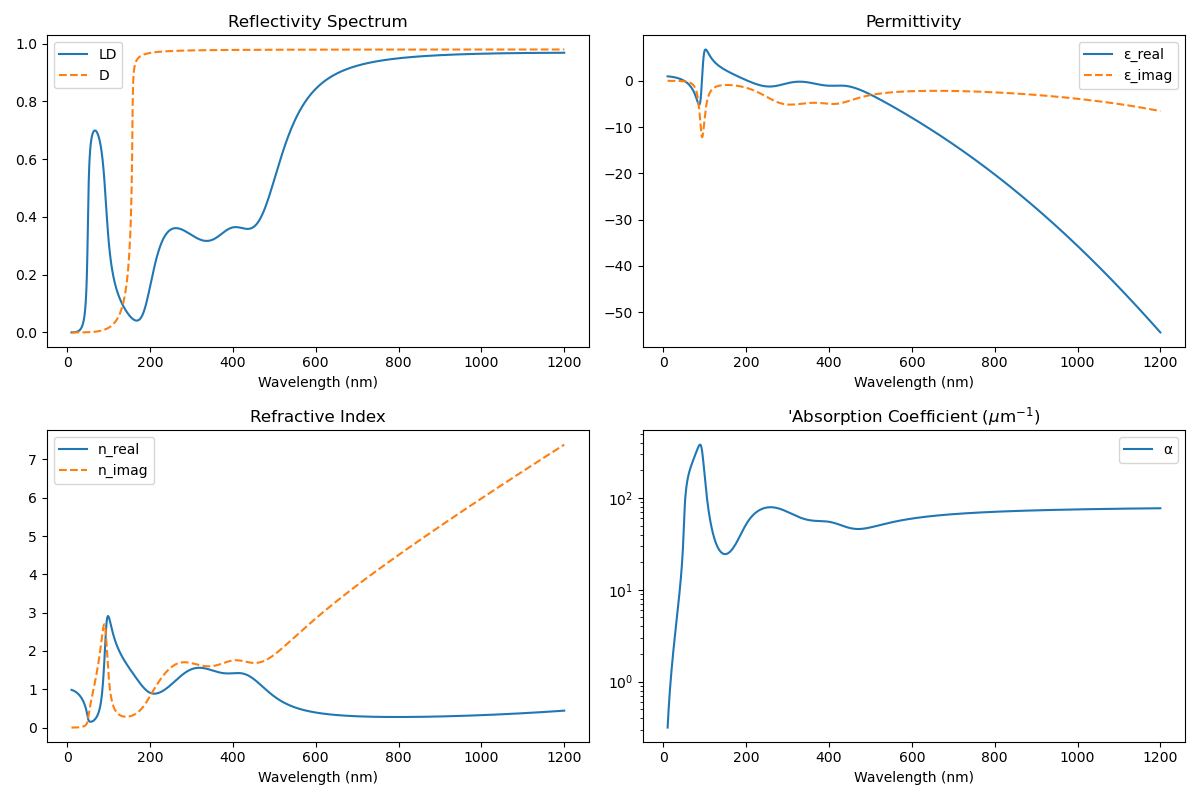
\includegraphics[width=0.85\linewidth]{figures/ch1/optical_au_spectrum_comparison_10_1200_RT.png}
  \caption{Spectrum comparison of optical models with optical parameters in the wavelength range of 10 to 1200 nm for Au. Both electron and lattice temperatures are set to 300 K.}
  \label{fig:ch1-au-spectrum-comparison}
\end{figure}

\begin{figure}[htbp]
  \centering
  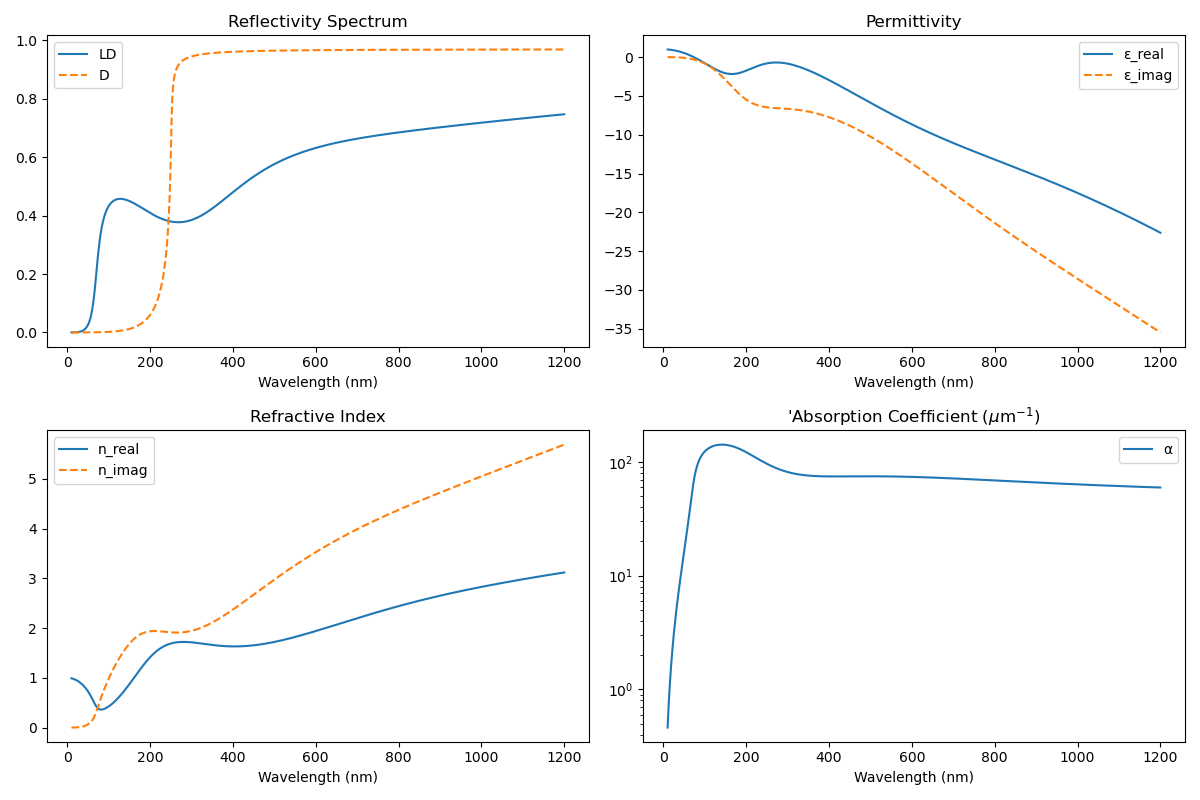
\includegraphics[width=0.85\linewidth]{figures/ch1/optical_ni_spectrum_comparison_10_1200_RT.png}
  \caption{Spectrum comparison of optical models with optical parameters in the wavelength range of 10 to 1200 nm for Ni. Both electron and lattice temperatures are set to 300 K.}
  \label{fig:ch1-ni-spectrum-comparison}
\end{figure}

Figures~\ref{fig:ch1-au-spectrum-comparison} and~\ref{fig:ch1-ni-spectrum-comparison} show the spectral consequences of this modelling choice. For Au the Lorentz--Drude correction is required to reproduce the interband response above the visible range, while for Ni the discrepancy between Drude-only and Lorentz--Drude fits is even more pronounced near the operating wavelength.
In the general case therefore we treat \(R\), \(\alpha\), and \(\delta_{opt}\) as wavelength- and temperature-dependent optical quantities rather than fixed room-temperature constants.

\section{Temperature dependent thermophysical parameters}
\label{sec:ch1-thermophysical-parameters}

A theoretical estimation of the $G$ factor was first proposed by Kaganov et al. \cite{Kaganov_1956} and further analysed by Qui \& Tien \cite{Qiu_1992}
\begin{equation}
  G(T_e) = \frac{\pi^2m_en_ec_s^2}{6\tau_e(T_e)T_e(t, \varrho, z)} \ ,
\end{equation}
where $m_e$ is the electron mass, $n_e$ the free electron density, and $c_s=\sqrt{B/\rho_m}$ the speed of sound in bulk material ($B$: bulk modulus, $\rho_m$: mass density).
This form emerges from treating electron--phonon scattering as the dominant thermalization channel in the TTM.
A more thorough investigation of the electron-phonon coupling in metals was conducted by Lin et al. \cite{Lin_2008} (e.g., eq.8 therein).

The heat capacity can be determined by the established formula \cite{Jiang_2005}
\begin{equation}
  C_e(T_e) = n_e \frac{\partial \langle \epsilon \rangle }{\partial T_e}\Biggl \vert_V = \int_\mathbb{R} \frac{\partial f(\epsilon, \mu, T_e)}{\partial T_e} g(\epsilon) \epsilon d\epsilon \ ,
\end{equation}
where V is the bulk material's volume and $\langle \epsilon \rangle$ is the energy ensemble average over the Fermi-Dirac distribution $f(\epsilon, \mu, T_e) \coloneqq [\exp\{(\epsilon - \mu)/k_BT_e\} +1]^{-1}$,
$\mu$ is the chemical potential and $g(\epsilon)$ denotes the electron density-of-states (DoS) at the energy level $\epsilon$.

The free electron heat conductivity is expressed by the Drude theory of metals as
\begin{equation}
  k_e(T_e) = \frac{1}{3} \langle v_e^2\rangle(T_e) \tau_e(T_e) C_e(T_e) \ ,
\end{equation}
where $\langle v_e^2 \rangle$ is the mean square of electron speed.\footnote{A more thorough theoretical description is provided by Jian and Tsai \cite{Jiang_2007}.}

To induce ablation in solid targets, a sufficiently high laser fluence is required. In such regimes, the $T_e$ could be $\sim T_F$ ($T_F^{\text{Au}} = 64.2 \times 10^3 K$), thus the Anisimov-Rethfeld formula is employed for the thermal conductivity\cite{Anisimov_1997}
\begin{equation}
  k_e(T_e, T_l) = \chi \frac{(\theta_e^2 + 0.16)^{5/4} (\theta_e^2 + 0.44) \theta_e}{(\theta_e^2 + 0.092)^{1/2}(\theta_e^2 + \eta \theta_l)} \ ,
\end{equation}
where $\theta_{e.l} = k_B T_{e,l}/ \epsilon_F$. The two constants are $\chi^{\text{Au}} = 353 \ Wm^{-1}K^{-1}$ and $\eta^{\text{Au}} = 0.16$ for gold. The asymptotic behavior of the heat conductivity is as follows:
\begin{itemize}
  \item $k_e(T_e ; \theta_e \gg 1) \sim T_e^{5/2}$, characteristic for low-density plasma.
  \item $k_e(T_e; \theta_e \ll 1) \sim T_e/ T_l$ (eq.14 in \cite{Chen_2001}).
\end{itemize}

As noted in  \cite{Jiang_2007}, at room temperature or higher, for Au phonons, the molar phonon heat capacity predicted by the quantum treatment (the Debye model) is similar to that predicted by the classical estimation (the Law of Dulong and Petit). Hence, the lattice heat capacity of gold in the calculation is reasonably considered as a constant (i.e., $C_l = const.$). Similarly, one could extend this approximation for other transition metals.

The electron heat conductivity can be expressed in a rational form, introduced by Yamashita \cite{Yamashita_2006}
\begin{equation}
  k_e(T_e,T_l) = k_{e0}\frac{B_L T_e}{A_e T_e^2 + B_L T_l}
  \label{eq:ch1-heat_conductivity_approx}
\end{equation}
where $k_{e0}$ is the electron heat conductivity at 300K, and $A_e$ and $B_L$ denote the electron-electron and electron-phonon scattering coefficients, respectively\footnote{$A_e$ and $B_L$ are estimated from variable angle spectral ellipsometry measurements of the refractive index and the extinction coefficient (e.g., describing absorption based on Forouhi-Bloomer dispersion relations \cite{Forouhi_1986}) in \cite{Fraggelakis_2021}.}.

The latter rational form approximates the Eidmann Model \cite{Eidmann_2000} and Matthiessen's rule \cite{Matthiessen_1864},
which combines two terms: the electron-ion (or electron-phonon, $k_{e-ph}$)
and the electron-electron ($k_{e-e}$) scattering contributions (reciprocal of conductivities $\propto$ collision rates)
\begin{equation}
  1/k_{tot} = 1/k_{e-ph} + 1/k_{e-e}.
  \label{eq:ch1-heat_conductivity_Matthiessen}
\end{equation}

In most cases, $k_e$ dominates $k_{(eq)}$ because free electrons contribute to the majority part of heat conduction.
For most metals, $k_l$ is usually taken to be 1\% of $k_e$ (i.e., $k_l \sim 0.01 k_e$).

Many of the ultrafast laser heating analyses have been carried out with a constant $G$ \cite{Kaganov_1956, Anisimov_1974, Hopkins_2013}.
However, due to the significant changes in the electron and lattice temperatures caused by high-power laser heating, $G$ should
be temperature dependent \cite{AlMalkawi_2018}.

Lin's group \cite{Lin_2008} in section II.C, defined the total electron scattering rate by
\begin{equation}
  \tau_e^{-1}(T_e, T_l) = A_eT_e^2 + B_LT_l.
  \label{eq:ch1-electron_scattering_rate}
\end{equation}
Chen et al. \cite{Chen_2005}, combining Lin et al.'s \cite{Lin_2008} scattering rate with equilibrium coupling at room temperature, $G_{RT}$,
showed that under the approximation of a temperature-independent DoS and a linearised energy exchange term, one obtains
\begin{equation}
  G(T_e,T_l) = G_{RT} \Bigl[\frac{A_e}{B_l}(T_e + T_l) + 1\Bigr]
  \label{eq:ch1-G_closed_formula}
\end{equation}
This closed-form is valid when
\begin{enumerate}[label=(\roman*)]
  \item the electronic DoS near the Fermi level is approximately constant,
  \item the two-temperature model remains in the linear-response regime, and
  \item higher-order inelastic processes are negligible.
\end{enumerate}

The heat capacity of electron proposed in a later work by Chen et al. \cite{Chen_2006}, is estimated as
\begin{equation}
  C_e = \left\{
  \begin{array}{ll}
    B_eT_e             & T_e < T_F/\pi^2                    \\
    2B_eT_e/3 + C_e'/3 & T_F/\pi^2 \leq T_e \leq 3T_F/\pi^2 \\
    Nk_B + C_e'/3      & 3T_F/\pi^2 \leq T_e \leq T_F       \\
    3Nk_B/2            & T_e \geq T_F
  \end{array}
  \right.
\end{equation}
where $B_e$ the coefficient for electron heat capacity ($Jm^{-3}K^{-2}$), $N$ the (conduction) electron number density ($m^{-3}$) and
\[
  C_e' = B_e T_F/\pi^2 + \frac{3Nk_B/2 - B_e T_F/\pi^2}{T_F - T_F/\pi^2}(T_e - T_F/\pi^2) \ .
\]

The temperature dependence of $C_e$ and $G$ is further investigated by Lin et al. \cite{Lin_2008} for representative metals (Al, Cu, Ag, Au, Ni, Pt, W, Ti) in the range of electron
temperatures typically realized in the ultrafast laser processing applications following the electron DoS and free-electron gas (FEG) model for comparison (e.g., figs.1,2 for Al in \cite{Lin_2008}).

At sufficiently low electron temperatures the Sommerfeld approximation of the electron heat capacity holds, \(C_e \approx \gamma T_e\),
but for temperature ranges of $\mathcal{O}(10^3-10^4)$K piecewise closures obtained from DoS data are employed:
\begin{subequations}\label{eq:ch1-ceg-piecewise}
  \begin{align}
    C_e(T_e) & =
    \begin{cases}
      p_{\mathrm{low}}(T_e),  & T_e \leq T_{\mathrm{th}} \, , \\
      p_{\mathrm{high}}(T_e), & T_e > T_{\mathrm{th}} \, ,
    \end{cases} \label{eq:ch1-ce-piecewise} \\
    G(T_e)   & =
    \begin{cases}
      q_{\mathrm{low}}(T_e),  & T_e \leq T_{\mathrm{th}} \, , \\
      q_{\mathrm{high}}(T_e), & T_e > T_{\mathrm{th}} \, ,
    \end{cases} \label{eq:ch1-g-piecewise}
  \end{align}
\end{subequations}
given empirical threshold temperatures ($T_{\mathrm{th}}$) for each metal in our database.
This choice preserves the low-temperature linear trend in Au while retaining the stronger nonlinear response required for materials such as Ni.

While our piecewise-polynomial fits of $G(T_e)$ capture the full nonlinearity present in the data (especially for Ni and Ti),
equation \ref{eq:ch1-G_closed_formula} provides a compact alternative that may be used in place of the high-order fits,
provided the above approximations hold and one uses the measured or computed $G_{RT}$ from DoS methods (as $G_{RT} \equiv G(T_e = T_\text{RT})$).

% \begin{figure}[H]
%   \centering
%   \includegraphics[width=0.80\linewidth]{figures/ch1/ceg_au_Ce_G_curves.png}
%   \caption{Piecewise polynomial fitting of electronic heat capacity (\(C_e\)) and electron-phonon coupling (\(G\)) for gold (Au) based on ab-initio density-of-states calculations.}
%   \label{fig:ch1-au-ce-g-curves}
% \end{figure}

% \begin{figure}[H]
%   \centering
%   \includegraphics[width=0.80\linewidth]{figures/ch1/ceg_ni_Ce_G_curves.png}
%   \caption{Piecewise polynomial fitting of electronic heat capacity (\(C_e\)) and electron-phonon coupling (\(G\)) for nickel (Ni) based on ab-initio density-of-states calculations.}
%   \label{fig:ch1-ni-ce-g-curves}
% \end{figure}

The effect of the electron DoS on the $G$ factor, which describes how the ab-intio temperature measurements were acquired using \href{https://www.vasp.at/}{VASP} is elaborated in the work by Fang et al. \cite{Fang_2012}.
In their first figure, which is included for completeness (Fig.\ref{fig:ch1-ce-g-literature}),
they highlight the linear dependence of $C_e(T_e)$ at low temperatures.

\begin{figure}[H]
  \centering
  \PublicFigureOmitted[0.85\linewidth]
  \caption{Electron temperature dependence of the electron heat capacity (left) and electron-phonon coupling factor (right) of Au. Solid lines show the results of the calculations performed with DoS obtained from VASP. Dashed lines show the commonly used approximations of the thermophysical material properties. \cite{Fang_2012}}
  \label{fig:ch1-ce-g-literature}
\end{figure}

\section{Laser power density \& volumetric heat source}
\label{sec:ch1-heat-source}

The expression for the time-dependent intensity distribution, inside the bulk material for both non-linear and linear
absorptions is provided by Jiang et al. \cite{Jiang_2004}, considering a gaussian laser beam with focus point being at the material surface,
\begin{equation}
  I(t, \mathbf{r}) = \sqrt{\frac{\beta_G}{\pi}} \frac{F}{\tau_p} (1 - R(t, \mathbf{r}; z=z_s))\times \exp \biggl\{ - \frac{x^2 + y^2}{R_0^2} - \beta_G \biggr(\frac{t}{\tau_p}\biggl)^2 - \int_{z_s}^z \alpha(t, \mathbf{r})dz \biggr\},
  \label{eq:ch1-intensity_distribution}
\end{equation}
where $\beta_G = 4\ln2$, $F$ is the laser fluence\footnote{
  Throughout the thesis we assume that the fluence, $F$,
  accounts accordingly for the number of constituent pulses
  so that the effective deposited energy is scaled consistently in single-pulse and double-pulse regimes.
}, $\tau_p$ the pulse duration, $R$ the (surface) reflectivity,
$R_0$ the FWHM of the laser beam and
$\alpha$ the (free-carrier) absorption coefficient\footnote{
  The beam attenuation includes additionally two-photon and three-photon absorption yielding quadratic and cubic nonlinearities respectively (eq.3 in \cite{Tsibidis_2019} or eq.15 in \cite{Driel_1987}).
}. Notice that the reflectivity is fixed at $z=z_s(\varrho)$.

Differentiating with respect to the depth coordinate, $z$, and mapping to cylindrical coordinates ($\varrho^2 = x^2 + y^2, \tan(\phi) = y/x$) utilizing the intensity's azimuthal isotropy we obtain the laser energy propagation loss
\begin{equation}
  \frac{\partial I(t,\varrho,z)}{\partial z}
  = \sqrt{\frac{\beta_G}{\pi}} \frac{F}{\tau_p} (1 - R(t,\varrho, z=z_s))
  e^{-\frac{\varrho^2}{R_0^2}}e^{-\beta_G \bigl(\frac{t}{\tau_p}\bigr)^2}e^{-\int_{z_s}^z\alpha dz}(-\alpha(t,\varrho,z))
  \label{eq:ch1-energy_propagation_loss_cylindrical}
\end{equation}
or
\begin{equation}
  \frac{\partial I(t,\varrho,z)}{\partial z} = -\alpha(t,\varrho,z) I(t,\varrho,z).
  \label{eq:ch1-energy_propagation_loss}
\end{equation}

Note that the attenuation of the laser beam along the propagation direction $z$ is more generally defined by the 1D ordinary differential equation:\cite{Driel_1987, Jiang_2007, Vaghasiya_2022}
\begin{equation}
  \frac{\partial I(t, \mathbf{r})}{\partial z} = - (\alpha_\text{BG} + \beta_\text{TPA} I(t, \mathbf{r}) + \Theta n) I(t, \mathbf{r}),
  \label{eq:ch1-energy_propagation_loss_general}
\end{equation}
where $\alpha_\text{BG}$ and $\beta_\text{TPA}$ denote the interband (BG: band-gap) and two-photon absorption coefficients, respectively.
$\Theta$ is the free-carrier absorption cross-section.
In metals, there is only the latter absorption, thereby we set $\alpha_\text{BG} = \beta_\text{TPA} = 0$ and define $\alpha \coloneqq \Theta n$ as the absorption coefficient, stemming from the Lorentz-Drude optical model
(eq.~\eqref{eq:absorption_FCA} with the ballistic correction in eq.~\eqref{eq:ch1-alpha-prime}).

Jiang \& Tsai show this is consistent with starting from the local energy loss of an incident beam to define the laser irradiation (heat source term in eq.~\eqref{eq:ch1-pttm}):\cite{Jiang_2007}
\begin{equation}
  S(t,\varrho,z) = - \frac{\partial I(t,\varrho,z)}{\partial z}.
  \label{eq:heat_source}
\end{equation}

As temporal envelopes, we enable selection of Gaussian (FWHM$=\tau_p$) and Lorentzian (HWHM$=\eta_L=\tau_p/2$),
with support for single-pulse (SP) or double-pulse (DP) modes.
\begin{equation}
  G(t; t_0) \equiv G\left(t; \mu = t_0, \sigma_t^2 = \tau_p^2/(2\beta_G) \right) \coloneqq \frac{1}{\tau_p}\sqrt{\frac{\beta_G}{\pi}} \exp\biggl\{ - \beta_G \Bigr(\frac{t - t_0}{\tau_p}\Bigl)^2 \biggr\} \ , \ \forall t_0 \in \mathbb{R} \ ,
  \label{eq:ch1-gaussian}
\end{equation}

\begin{equation}
  L(t; t_0) \equiv L(t; \mu = t_0, \eta_L = \tau_p/2) \coloneqq \frac{2}{\pi \tau_p} \biggl[ 1 + 4 \Bigr(\frac{t - t_0}{\tau_p}\Bigl)^2  \biggr]^{-1} \ , \ \forall t_0 \in \mathbb{R} \ .
  \label{eq:ch1-lorentzian}
\end{equation}

It is common in the literature to introduce artificial propagation lags; offsets place the Gaussian envelope inside the simulation time window.
For instance, $G(t; t_0=t_c)$ is the temporal distribution of a reference Gaussian envelope centred at $t_c = n\tau_p$ with variance $\sigma^2 \coloneqq \tau_p^2/(2\beta_G)$ and FWHM$\coloneqq 2 \sqrt{2\ln(2)} \sigma = \tau_p$,
such as $\tau_pG(0) \sim \exp\{-\beta_G n^2\}$ which is effectively zero for $n=3$ ($\approx 10^{-11}$).
For any dimensionality of the heat source (1--D, 2--D, 3--D) we use $n=3$, although in the 1--D case Chen et al. \cite{Chen_2010} follow the convention $n=2$.

\noindent
Then, the intensity of a constituent laser beam is defined as
\begin{equation}
  I_1(t,\varrho,z) \coloneqq F E_\text{tot}(t) \exp\Bigl\{ -\frac{\varrho^2}{R_0^2} \Bigr\} \exp\Bigl\{ - \int_{z_s}^z \alpha(t,\varrho,z)dz \Bigr\},
  \label{eq:ch1-intensity_laser_beam}
\end{equation}
where $E_\text{tot}$ is a sum of one (or two) Gaussian or Lorentzian pulses,
centred at $t_c$ for a single pulse and $t_c + t_d$ under double-pulse mode.

\noindent
Accounting for the surface reflectivity we obtain
%
\begin{equation}
  I_\text{(ULP)}(t,\varrho,z) = (1 - R(t,\varrho,z_s)) I_1(t,\varrho,z).
  \label{eq:ch1-intensity_reflect_I_1}
\end{equation}
%
Assuming the optical penetration depth is much smaller than the target's thickness, i.e. $\delta_{opt} \ll L_z$, we can assert depth-independent absorption (Beer-Lambert attenuation).
Under this condition, we obtain an expression for the laser heat source (under ULP regime)
\begin{equation}
  S_\text{(ULP)}(t,\varrho,z) \equiv \alpha I_\text{(ULP)}(t,\varrho,z) \approx \alpha F (1 - R(t,\varrho,z_s)) E_\text{tot}(t) f(\varrho; R_0) \exp\{- \alpha (z - z_s)\},
  \label{eq:ch1-volumetric_heat_source}
\end{equation}
where $f(\varrho; R_0)$ is the transverse beam profile with constant spot radius $w = R_0$,
assuming infinite depth of focus or, equivalently, infinite Rayleigh length ($z_R \rightarrow \infty$ in eq.~\eqref{eq:ch1-beam_propagation}):
\begin{equation}
  f(\varrho; w(z,t)= R_0) = \left. \exp\Bigl\{ - \frac{\varrho^2}{w^2(z,t)} \Bigr\} \right|_{w=R_0}.
  \label{eq:ch1-beam_profile}
\end{equation}

Considering the effects of ballistic motion and hot electron diffusion which extend the absorbed energy into greater depth of the electrons, drastically for metals, Wellershoff et al. \cite{Wellershoff_1999} and Hohlfeld et al. \cite{Hohlfeld_2000} introduced these contributions into the laser heat source by adding the ballistic range to the optical penetration path.
This results in the axisymmetric volumetric heat source
(with $\alpha'$ from eq.~\eqref{eq:ch1-alpha-prime} and $b(L_z; \alpha')$ from eq.~\eqref{eq:ch1-thickness-factor})
\begin{equation}
  S(t, \varrho, z) \coloneqq \alpha' b(L_z; \alpha') [1 - R] I_1(t,\varrho,z; \alpha'),
  \label{eq:ch1-ulp_heat_source}
\end{equation}
with $R=R(\varrho, z=z_s; T_e, T_l)$ being the surface reflectivity, which inherits the axisymmetry of the laser beam.

\subsection{Dimensionality Reductions - Slicing vs Integrating}

There are two consistent ways to reduce 3D to lower dimensions, integrate over the suppressed coordinate
(gives a surface/line source) or slice (evaluate at a representative value, typically the beam centre).
The appropriate approach depends on the solver's state variables (volumetric vs surface parameters).
In this part of the thesis, we reconcile both in the axisymmetric context.

\subsubsection{From 3D to 2D under axial symmetry}

Let the transverse profile be factorable $I_\text{total}(t,\varrho,z) = F E_\text{tot}f(\varrho)e^{-\alpha(z-z_s)}\mathds{1}\{z \geq z_s\}$
for simplicity (Gaussian radial profile $f(\varrho) = \exp\{ -\varrho^2/(2\sigma_r^2) \}$, where $\sigma_r \coloneqq w_0/\sqrt{2}$).

\paragraph{(A) Integrate over one suppressed coordinate (surface/line source).}
If we collapse the $\phi$ coordinate we form a 2D source per unit length in $\varrho-z$ (units W$\cdot$m$^{-2}$):
\begin{equation}
  \widetilde{S}_\text{2D} = \int_{0}^{2\pi} S_\text{3D}(t, \varrho, \phi, z) \varrho d\phi = 2\pi \; \varrho \; \alpha' \; b(\alpha') \; (1-R) \; F \; E_\text{tot}(t) \; f(\varrho) \; e^{-\alpha'(z-z_s)} \; \mathds{1}\{z \geq z_s\}\ .
\end{equation}
This object is the power per unit length in $z$ per radial distance $\varrho$. Note the $2\pi\varrho$ prefactor from converting from Cartesian to cylindrical integration).
It is the appropriate form when the solver uses line/surface capacities that already incorporate the radial Jacobian.
\vspace{10pt}

\paragraph{(B) Slice / representative volumetric source (volumetric 2D).}
If the solver expects a volumetric source in the 2D ($x=\varrho,z$) plane (units W$\cdot$m$^{-3}$),
a widely used practical choice is to evaluate the 3D source at the representative azimuth (e.g., $\phi=0$)
and not integrate (this is analogous to the Cartesian slice at $y=0$):
\begin{equation}
  S_\text{2D}(t,\varrho,z) \equiv S_\text{3D}(t,\varrho,z) = \alpha' \; b(\alpha') \; (1-R) \; F \; E_\text{tot}(t) \; f(\varrho) \; e^{-\alpha'(z-z_s)} \; \mathds{1}\{z \geq z_s\} \ .
\end{equation}
The $2\pi\varrho$ extra factor is not absent here as we integrate over the angle variable, keeping pointwise volumetric units.\\
Namely, $S_\text{2D}$ is the volumetric power density in the slice/meridian plane and is suitable when the solver retains volumetric capacities $C_v$ (J$\cdot$m$^{-3}$$\cdot$K$^{-1}$).

  \subsubsection{From 2D to 1D (depth-only)}

  \begin{enumerate}
    \item Integrated power per unit depth (units: W$\cdot$m$^{-1}$):
          \begin{equation}
            \widetilde{S}_\text{1D}(t,z) = \int_\text{transverse} S_\text{3D} (t, \mathbf{r}) dA =  A_\text{eff}\;\alpha'\;b(\alpha')\;(1-R)\;F\;E_\text{tot}(t)\;e^{-\alpha'(z-z_s)} \; \mathds{1}\{z \geq z_s\} \ ,
          \end{equation}
          where $A_\text{eff} \coloneqq \iint f(x,y)dxdy$ is the effective beam area.
    \item Area-averaged volumetric source for a 1D depth model (units: W$\cdot$m$^{-3}$):
          \begin{equation}
            S_\text{1D}(t,z) = \frac{\widetilde{S}_\text{1D}(t,z)}{A_\text{eff}} = \alpha'\;b(\alpha')\;(1-R)\;F\;E_\text{tot}(t)\;e^{-\alpha'(z-z_s)} \; \mathds{1}\{z \geq z_s\} \ .
          \end{equation}
          This is identical in form to the usual depth-only exponential source in many TTM implementations (c.f. Ren et al. (2011) \cite{Ren_2011}).
  \end{enumerate}
  Therefore, we follow the slicing approach since we are supplied with volumetric capacities ($C_e(T_e)$ and $C_l \coloneqq \rho_l \cdot c_l$).

  Below are shown comparative figures adopted from Chen et al. \cite{Chen_2002}
  simulating with the dual-hyperbolic 1D and 3D TTM (eqs.6-12 therein) using a fourth-order finite-difference scheme with regular grid mesh.

  \begin{figure}[H]
    \centering
    % Subfigure (a)
    \subfloat[Electron temperature profile across the thickness ($z$-axis) at $\varrho=0$ for a 100-nm gold film\\($\tau_p=100$~fs, $F=4107$~J/m$^2$, $w_0=500$~nm). \cite{Chen_2002}]{
      \PublicFigureOmitted[0.44\linewidth]
      \label{fig:ttm-Te-profile}
    }
    \hfill
    % Subfigure (b)
    \subfloat[Temporal evolution of electron ($T_e$) and lattice ($T_l$) temperatures at the front surface centre ($\varrho=0, z=0$) for a 100-nm gold film ($\tau_p=100$~fs, $F=4107$~J/m$^2$, $w_0=2.0$~$\mu$m). \cite{Chen_2002}]{
      \PublicFigureOmitted[0.44\linewidth]
      \label{fig:ttm-temp-history}
    }
    \caption{Comparison of spatial and temporal temperature distributions in a 100-nm gold film predicted by the Two-Temperature Model (TTM).}
    \label{fig:ttm_1d_vs_3d}
  \end{figure}

  \section{Two-temperature model variants and model selection}
  \label{sec:ch1-ttm-variants}

  Classical Fourier heat conduction remains adequate when the laser pulse duration exceeds both the electron and lattice relaxation times, so the irradiated metal may be treated as a single equilibrium medium. Under ultrafast illumination, however, the two subsystems decouple temporally and a two-step description becomes necessary. Anisimov et al.\ first established the parabolic two-step framework for this regime \cite{Anisimov_1974} which was advanced further by Fujimoto et al.\ \cite{Fujimoto_1984},
  while later work introduced hyperbolic heat-flux corrections for finite-speed thermal transport and dual-subsystem relaxation effects \cite{Qiu_1992, Bai_1995, Chen_2001}.

  The parabolic one-step model (POS) therefore represents the classical laser-heating limit:
  \begin{equation*}
    \rho_m c_p \frac{\partial T}{\partial t} = \nabla \cdot (k \nabla T) + S \, .
  \end{equation*}
  % [NOTATION: changed \rho \rightarrow \rho_m per chapter convention outside §1.5]
  Here \(\rho_m\) denotes the material density and \(c_p\) the isobaric specific heat capacity. The POS assumes instantaneous Fourier transport and remains appropriate when the pulse duration exceeds substantially the values of electron and lattice relaxation times, i.e., \(\tau_p \gg \tau_e\) and \(\tau_p \gg \tau_l\), which corresponds to the long-pulse or continuous-wave heating limit \cite{Tzou_2014ch1}.

  The parabolic two-step model (PTS) separates the electron and lattice temperatures while retaining Fourier conduction in the electron subsystem. In the notation of this thesis, the coupled PTS system has already been introduced in \eqref{eq:ch1-pts}. This model is appropriate when \(\tau_p > \tau_e\) but \(\tau_p < \tau_l\), so the electrons thermalise during the pulse whereas the lattice responds on a delayed timescale \cite{Anisimov_1974,Qiu_1992}. The pTTM adopted in \S\ref{sec:ch1-ultrashort} starts from this structure and extends it by retaining Fourier conduction in the lattice subsystem.

  The hyperbolic one-step model (HOS) or Maurer's model \cite{Maurer_1969} replaces Fourier's law by the Maxwell--Cattaneo--Vernotte relation,\cite{Vernotte_1958,Majchrzak_2012}\footnote{
    Cattaneo introduced the thermal relaxation characteristic time $\tau_0$ \cite{Cattaneo_1948}, which is interpreted by Chandrasekharaiah as \emph{the
      time lag required to establish steady heat conduction in a volume element once a
      temperature gradient has been imposed across it} \cite{Chandrasekharaiah_1998},
    i.e., the time needed to reach thermodynamic stability.
  }
  \begin{align*}
    \rho_m c_p \frac{\partial T}{\partial t}                   & = -\nabla \cdot \mathbf{q} + S \, , \\
    \mathbf{q} + \tau_e \frac{\partial \mathbf{q}}{\partial t} & = -k_{eq}\nabla T \, ,
  \end{align*}
  % [NOTATION: changed \rho \rightarrow \rho_m per chapter convention outside §1.5]
  which leads to the finite thermal-wave speed \(c_T = \sqrt{k_{eq}/(\rho_m c_p \tau_e)}\). In the single-temperature setting this correction becomes relevant once the effective relaxation time is no longer negligible over the pulse timescale, which is commonly associated with \(\tau_p \sim \tau_l\) in lattice-dominated heating problems \cite{Majchrzak_2012, Mochnacki_2013}.

  The hyperbolic two-step model (HTS) then introduces the electron heat-flux relaxation explicitly:\cite{Qiu_1993}
  \begin{align*}
    C_e \frac{\partial T_e}{\partial t}                            & = -\nabla \cdot \mathbf{q}_e - G(T_e - T_l) + S \, , \\
    \mathbf{q}_e + \tau_e \frac{\partial \mathbf{q}_e}{\partial t} & = -k_e \nabla T_e \, ,                               \\
    C_l \frac{\partial T_l}{\partial t}                            & = G(T_e - T_l) \, .
  \end{align*}
  It accounts for the finite electron relaxation time and reduces to the PTS in the limit \(\tau_e \to 0\).
  The HTS is therefore the appropriate extension when \(\tau_p \sim \tau_e\).

  The dual-hyperbolic two-step model (DHTS) extends the HTS by retaining a separate lattice heat flux,
  \begin{align*}
    C_e \frac{\partial T_e}{\partial t}                            & = -\nabla \cdot \mathbf{q}_e - G(T_e - T_l) + S \, , \\
    \mathbf{q}_e + \tau_e \frac{\partial \mathbf{q}_e}{\partial t} & = -k_e \nabla T_e \, ,                               \\
    C_l \frac{\partial T_l}{\partial t}                            & = -\nabla \cdot \mathbf{q}_l + G(T_e - T_l) \, ,     \\
    \mathbf{q}_l + \tau_l \frac{\partial \mathbf{q}_l}{\partial t} & = -k_l \nabla T_l \, .
  \end{align*}
  The DHTS assigns finite wave speeds to both subsystems and is therefore the most general TTM variant before drift-velocity corrections are introduced. It becomes necessary when both electron and lattice relaxation effects are comparable with the pulse timescale \cite{Chen_2001}.

  The semiclassical two-step model (STS) goes one step further by incorporating the electron drift velocity generated by the combined action of the electric field and the hot-electron kinetic pressure. Chen et al.\ introduced this extension for very short, high-intensity pulses, where drift transport becomes comparable with diffusion and therefore cannot be neglected in the electron energy balance \cite{Chen_2006}.

  Table~\ref{tab:ch1-ttm-taxonomy} summarises the governing structure, wave-speed characteristics, and validity range of the principal TTM variants discussed above, following the Qiu--Tien taxonomy in \cite{Qiu_1992} and the later classification of Alexopoulou et al. Figure~\ref{fig:ch1-ttm-taxonomy} shows the corresponding model interrelationship.

  % =========================================================
  % TTM taxonomy table
  % =========================================================
  \begin{table}[htbp]
    \centering
    \small
    \caption{Summary of one- and two-temperature model variants for ultrashort-pulse laser heating of metals. The table follows the taxonomy introduced by Qiu and Tien and the later literature classification adopted in the field.}
    \label{tab:ch1-ttm-taxonomy}
    \renewcommand{\arraystretch}{1.35}
    \setlength{\tabcolsep}{5pt}

    \resizebox{\linewidth}{!}{%
      \begin{tabular}{@{}>{\centering\arraybackslash}m{1.5cm}
        >{\raggedright\arraybackslash}m{5.7cm}
        >{\centering\arraybackslash}m{3.4cm}
        >{\centering\arraybackslash}m{4.4cm}
        >{\centering\arraybackslash}m{2.5cm}@{}}
        \toprule
        \rowcolor{gray!20}
        \textbf{Model} & \textbf{Governing equations}                                       & \textbf{Thermal-wave speed} & \textbf{Validity regime}                  & \textbf{References} \\
        \midrule
        POS            & \(\rho_m c_p \dot{T} = \nabla \cdot (k \nabla T) + S\)             & Infinite                    & \(\tau_p \gg \tau_e,\ \tau_p \gg \tau_l\) & \cite{Tzou_2014ch1} \\
        \midrule
        PTS            & \makecell[l]{Two coupled energy equations                                                                                                                          \\ for \(T_e\) and \(T_l\);\\ Fourier conduction retained in\\ the electron subsystem} & Infinite & \(\tau_p > \tau_e,\ \tau_p < \tau_l\) & \cite{Anisimov_1974,Fujimoto_1984,Qiu_1992} \\
        \midrule
        HOS            & \makecell[l]{\(\rho_m c_p \dot{T} = -\nabla \cdot \mathbf{q} + S\)                                                                                                 \\ \(\mathbf{q} + \tau_e \dot{\mathbf{q}} = -k_{eq}\nabla T\)} & \(\displaystyle c=\sqrt{\frac{k_{eq}}{\rho_m c_p \tau_e}}\) & \makecell[c]{Single-temperature setting;\\ effective relaxation\\ not negligible, often \(\tau_p \sim \tau_l\)} & \cite{Maurer_1969,Vernotte_1958,Majchrzak_2012,Mochnacki_2013} \\
        \midrule
        HTS            & \makecell[l]{Electron energy balance with                                                                                                                          \\ hyperbolic flux +\\ lattice source balance\\ without lattice flux} & \(\displaystyle c_e=\sqrt{\frac{k_e}{C_e\tau_e}}\) & \(\tau_p \sim \tau_e\) & \cite{Qiu_1992,Qiu_1993} \\
        \midrule
        DHTS           & \makecell[l]{Electron and lattice both with                                                                                                                        \\ hyperbolic heat-flux relations} & \makecell[c]{\(\displaystyle c_e=\sqrt{\frac{k_e}{C_e\tau_e}}\)\\[0.6em] \(\displaystyle c_l=\sqrt{\frac{k_l}{C_l\tau_l}}\)} & \makecell[c]{\(\tau_p \sim \tau_e,\)\\ \(\tau_p \sim \tau_l\)} & \cite{Chen_2001} \\
        \midrule
        STS            & \makecell[l]{DHTS augmented by electron                                                                                                                            \\ drift velocity and\\ hot-electron pressure /\\ electric-field effects} & \makecell[c]{Finite in both\\ subsystems} & \makecell[c]{Very short,\\ high-intensity pulses\\ where drift transport\\ is non-negligible} & \cite{Chen_2006} \\
        \bottomrule
      \end{tabular}%
    }
  \end{table}

  % =========================================================
  % Relaxation times used in hyperbolic TTM / DHTM
  % =========================================================

  \begin{table}[htbp]
    \centering
    \small
    \caption{Reported relaxation times used in Maxwell--Cattaneo--Vernotte-type electron and lattice heat-flux relations in hyperbolic one-step, hyperbolic two-step, and dual-hyperbolic two-temperature models.}
    \label{tab:ch1-relaxation-times-hyperbolic-ttm}
    \renewcommand{\arraystretch}{1.35}
    \setlength{\tabcolsep}{5pt}

    \resizebox{\linewidth}{!}{%
      \begin{tabular}{@{}>{\raggedright\arraybackslash}m{2.8cm}
        >{\raggedright\arraybackslash}m{4.7cm}
        >{\centering\arraybackslash}m{2.2cm}
        >{\centering\arraybackslash}m{2.2cm}
        >{\raggedright\arraybackslash}m{3.8cm}
        >{\centering\arraybackslash}m{2.1cm}@{}}
        \toprule
        \rowcolor{gray!20}
        \makecell[l]{\textbf{Material /}            \\ \textbf{system}} &
        \textbf{Model context}      &
        \textbf{\(\tau_e\) (ps)}    &
        \textbf{\(\tau_l\) (ps)}    &
        \textbf{Method / basis}     &
        \textbf{Reference}                          \\
        \midrule

        Au thin film                &
        \makecell[l]{Hyperbolic two-step / electron \\ MCV flux} &
        \(0.04\)                    &
        ---                         &
        \makecell[l]{Adopted as electron            \\ heat-flux relaxation time} &
        \cite{Qiu_1992,Qiu_1993}                    \\
        \midrule

        Au thin film                &
        \makecell[l]{Dual-hyperbolic two-step       \\ model} &
        \(0.04\)                    &
        \(0.8\)                     &
        \makecell[l]{Canonical DHTS input           \\ values for Au} &
        \cite{Chen_2001}                            \\
        \midrule

        Au thin film                &
        \makecell[l]{Later DHTS / hyperbolic-       \\ TTM reuse} &
        \(0.04\)                    &
        \(0.8\)                     &
        \makecell[l]{Reused from Chen--Beraun       \\ gold-film model} &
        \cite{Majchrzak_2012}                       \\
        \midrule

        Cr thin film                &
        \makecell[l]{Dual-hyperbolic two-step       \\ model for bilayers} &
        \(6.8\times10^{-3}\)        &
        \(0.136\)                   &
        \makecell[l]{Reported as model-input        \\ values for Cr} &
        \cite{Niu_2009}                             \\
        \midrule

        \makecell[l]{Au/Cr bilayer} &
        \makecell[l]{Bilayer hyperbolic two-step    \\ model} &
        \makecell[c]{Au: \(0.04\)                   \\ Cr: \(6.8\times10^{-3}\)} &
        \makecell[c]{Au: ---                        \\ Cr: \(0.136\)} &
        \makecell[l]{Layerwise hyperbolic           \\ model inputs} &
        \cite{Niu_2009}                             \\
        \bottomrule
      \end{tabular}%
    }
  \end{table}

  \begin{figure}[htbp]
    \centering
    \PublicFigureOmitted[0.60\linewidth]
    \caption{Taxonomy and interrelationship between laser heating models, adapted from Qiu and Tien \cite{Qiu_1992}.}
    \label{fig:ch1-ttm-taxonomy}
  \end{figure}

  The present thesis focuses on femtosecond laser-matter interaction in metals,
  with pulse durations of $\mathcal{O}(10^4)$ fs ($\tau_p \sim 10$ ps) and representative materials including Au, Ni, Ti, Cu, and 100Cr6 steel.
  In this regime the electron relaxation time is typically of $\mathcal{O}(10)$ fs,
  whereas the lattice relaxation time remains on the picosecond-to-nanosecond scale (see table~\ref{tab:ch1-ttm-taxonomy} for more details).
  Consequently, \(\tau_p > \tau_e\) but \(\tau_p < \tau_l\), which places the simulations in the domain where the PTS family is physically appropriate. Hyperbolic corrections become central once \(\tau_p \sim \tau_e\), but that is not the primary operating regime of the present work \cite{Tzou_2014ch5, Alexopoulou_2023, Zhang_2015}.

  The retained damage indicator is therefore thermal, based on the maximum lattice temperature. Extensions that resolve interference-imposed sources, melt flow, capillary response, and morphology evolution are well documented elsewhere \cite{Fraggelakis_2021,Tsibidis_2012,Bonse_2020,M_ller_2020,Rudenko_2016,Colombier_2020}, but remain outside the pTTM state model investigated here.
